\documentclass[12pt,english]{article}
\usepackage[verbose,letterpaper,hmargin={2.4cm,2.4cm},vmargin={2.4cm,2.4cm}]{geometry}
\usepackage[mathlines]{lineno} 
\linenumbers
\usepackage[nodisplayskipstretch]{setspace}
\usepackage{amsmath}
\usepackage{amsfonts}
\usepackage{bm}
\usepackage{graphicx}
\usepackage[round,comma,authoryear]{natbib}
\usepackage{color, soul}
\usepackage{fancyvrb}
\usepackage{verbatim}
\usepackage{indentfirst}
\usepackage[format=plain,justification=raggedright,labelsep=period,font={stretch=1.9}]{caption}
\usepackage[pdftex,hidelinks]{hyperref} 
\usepackage{rotating}
\usepackage[compact]{titlesec}
\titleformat{\section}[display]{\normalfont\bfseries}{}{0em}{\centering}
\titleformat{\subsection}[display]{\normalfont\itshape}{}{0em}{\centering}
\bibliographystyle{ecology}
\setlength{\bibsep}{0.0pt}
\bibpunct{(}{)}{,}{a}{}{,}
\setlength{\jot}{-1.2ex}
\setstretch{1}
\widowpenalty 2
\clubpenalty 2
\usepackage{etoolbox}
\AtBeginEnvironment{tabular}{\doublespacing}
\makeatletter
\let\@fnsymbol\@arabic
\makeatother
\title{Improved state-space models for inference about 
spatial and temporal variation in abundance from count data}

\author{Jeffrey A. Hostetler\thanks{Migratory Bird Center, Smithsonian 
Conservation Biology Institute, National Zoological Park, MRC 5503, 
Washington, DC 20013-7012} \textsuperscript{,}\footnote{Email: \href{mailto:hostetlerj@si.edu}{hostetlerj@si.edu}}
   \and Richard B. Chandler\footnote{USGS Patuxent Wildlife Research Center 
        Laurel, MD 20708} \textsuperscript{,}\thanks{Current address: Warnell School of
     Forestry and Natural Resources, University of Georgia}        
}
\date{} 
\begin{document}
\maketitle
\vspace{-1cm}
\begin{spacing}{1.9}
\begin{flushleft}
\abstract{
Models of population dynamics 
are frequently used for purposes such as testing 
hypotheses about density dependence and predicting species' responses 
to future environmental change or conservation actions. Fitting models
of population dynamics to field data is challenging because most data
sets are characterized by observation error, which
can inflate estimates of process variation if ignored.  
Recently, state-space models have been developed to deal with this problem
by directly modeling both the observation error and the ecological
process of interest.
Conventional state-space models, however, have
several important limitations: (1) they assume that random effects are
Gaussian distributed, which implies that abundance can be negative and
that false positive observation errors are equally likely as false negative
errors; (2) they do not admit spatial variation in
population dynamics; and (3) some of the parameters of the model are not
estimable. We demonstrate how each of these problems can be
resolved using a class of hierarchical models proposed by
\citet[Biometrics]{dail_madsen:2011} 
that attributes observation error to imperfect detection.
We expand this class of models to accommodate classical growth
models (e.g. exponential and Ricker-logistic), zero-inflation,
and random effects. 
We also present methods for forecasting
population size under future environmental conditions. Implementation
of these ideas is possible using either frequentist or Bayesian
methods, as demonstrated by accompanying {\bf R} and {\bf JAGS} code. 
Results of a simulation study suggest that bias is 
negligible and coverage
nominal for the proposed model extensions. An analysis of data from
the North American Breeding Bird Survey highlights how these methods
can be readily applied to existing data, but it also suggests 
that precision will be low when direct information about detection
probability (such as is collected using distance sampling or
replicated counts) is lacking.
}

\textit{Key words}: abundance, Dail and Madsen model, density-dependence,
detectability, Gompertz-logistic, immigration, % model
population dynamics, Ricker-logistic, zero-inflated % model

%\vspace{0.5cm}

\section*{Introduction}
Models of population dynamics are vital in both theoretical and
applied ecological research. For instance, 
the importance and existence of phenomenon such as
density-dependent population regulation, population cycling, and
spatial synchrony have been studied by comparing data from natural
populations with theoretical models
\citep{may:1975,turchin:1990,bjornstad_etal:1999}. 
In applied contexts, population models are used for estimating extinction risk 
\citep{nadeem_lele:2011,hostetler_etal:2012} and for predicting the %schoener_spiller:1992,
effects of future environmental conditions or conservation actions on
population size \citep{jamieson_brooks:2004,hatfield_etal:2012}.

Two challenges are routinely encountered when trying to fit models %Several
of population dynamics to data from field studies. 
First, deterministic models of population dynamics are generally inadequate due to process %virtually always
variation, the stochasticity in demographic parameters and environmental % inherent
conditions \citep{bjornstad_grenfell:2001,saether_engen:2002}.
Second, abundance---the natural state variable in studies
of population dynamics---can rarely be observed perfectly in field
studies because of observation error, such as imperfect
detection \citep{link_nichols:1994,kery_etal:2009}.

Recently developed state-space models 
have made it possible to
study population dynamics while accounting for both process variation
and observation error \citep{devalpine_hastings:2002,
  buckland_etal:2004, dennis_etal:2006}. Classical state-space
models are time series models in which the true state of the
system (e.g. population size during each year) is modeled as a latent 
process, and the observed data are modeled conditional on this process
and the observation error. One reason for the widespread adoption of
state-space models in ecology is that failure to account for 
observation error can bias estimators of abundance and
population growth parameters. For instance, the strength of
density dependence will be overestimated if observation error is
ignored \citep{link_nichols:1994,shenk_etal:1998}.

A simple state-space model can be described as follows.
Let $N_t$ be the abundance of a species during year $t$, for
$t=1,\hdots,T$, and let $X_t$ be
the observed data, which differs from $N_t$ due to observation error,
a random effect denoted $\zeta_t$. Temporal variation in $N_t$ is
modeled using a population growth model, $\mu(N_{t-1})$
and random process variation denoted $\eta_t$.
The growth model may be density-dependent, as in the case of the 
Ricker-logistic model (henceforth Ricker model), or it might be 
density-independent, such as when growth
is exponential. %% Exponential or geometric?
A generic model can be written: 
\begin{linenomath*}
\begin{gather}
  \label{eq:ss1}
  \begin{align}
    N_1 &= x_0 \nonumber \\ %X_1
N_t &= \mu(N_{t-1}) + \eta_{t-1} \quad \text{for} \; 
t=2,\hdots,T  \\
X_t &= N_t + \zeta_t \qquad \qquad \;\, \text{for} \;
t=1,\hdots,T. \nonumber 
  \end{align}
\end{gather}
\end{linenomath*}
where $x_0$ is the model for initial abundance.  In classical
state-space models, the two sets of random effects
are assumed to be i.i.d. Gaussian variables: 
$\eta_t \sim \mathrm{N}(0, \sigma)$ and
$\zeta_t \sim \mathrm{N}(0, \tau)$. 
The process variation associated with $N_1$ is often ignored, or
the population is assumed to be at equilibrium such that the $N_1$ can
be regarded as an outcome of the equilibrium distribution.

Even though state-space models such as that shown in Eq.~\ref{eq:ss1}
overcome many of the limitations associated with the application of
classical models of population dynamics, 
several problems exist. 
The assumption that random effects are Gaussian distributed makes it
easier to estimate parameters because methods such as the Kalman
filter can be applied 
\citep{dennis_etal:2006}; however, 
these models effectively assume that abundance can be take on any
real value, and hence they can predict negative values of abundance. 
Transforming the count data and the underlying abundance variables 
do little to resolve these issues \citep{ohara_kotze:2010}.

With respect to the observation error, the Gaussian assumption
implies that false positive detections are
equally likely as false negatives, a pattern inconsistent with most
findings \citep{miller_etal:2011}. 
A more likely form of observation error, and one that has been recognized for well
over a century, results from failing to detect individuals that are
present. Imperfect detection may be attributable to
characteristics of the species under study, such as it being present but unavailable for detection,
or to individuals being available but missed by the ecologist collecting the data in the field.
Although a vast number of methods have been devised to account for 
this form of observation error, rarely have these methods been
integrated into state-space models of population dynamics. 
Of the exceptions that exist, none provide software to facilitate model fitting 
\citep{buckland_etal:2004}.

Other limitations of state-space models, as commonly applied in ecology,
include the failure to admit spatial variation in abundance and
the fact that some parameters are not identifiable
\citep{polansky_etal:2009}. 
Ignoring spatial variation reduces the scope of the
inferences, reduces the information about the parameters of interest,
and can lead to underestimation of variances \citep{dennis_etal:2010}.
Even more problematic is the issue that without some form of replication in the first year, 
abundance cannot be estimated without making strong assumptions about 
the initial distribution. 
For example, practitioners either assume that there is no
observation error in the first year ($x_0 = X_1$), or they assume the population is
at equilibrium, which may defeat the purpose of many studies of
population dynamics. 

Several extensions of state-space models have been proposed to
overcome the limitations described above. \citet{devalpine_hastings:2002} and
\citet{brooks_etal:2004} described methods for fitting models with non-Gaussian
distributions for the process and observation errors. An observation model %with
%more intuitive interpretations, such as those that 
explicitly modeling
detection probability has been proposed by 
\citet{kery_etal:2009}. \citet{lele_etal:1998} and 
\citet{kery_etal:2009} developed models allowing for inference about
spatial and temporal variation in abundance, and their developments
also resolved the problems of non-identifiability for the parameters
of the initial state at time $t=1$. Of these extensions, only
the work by \citet{kery_etal:2009} addressed several of these limitations
simultaneously; however, their model did not include serial
dependence, which is a hallmark of classical population growth models as well as state-space models. 

In this paper, we focus on the model of \citet[henceforth the DM model]{dail_madsen:2011}
that resolves each of the problems outlined above. 
Our aim is to extend the
model to accommodate classical models of population growth and
to handle several features common to ecological
time series, such as excess zeros and unexplained random variation. 
Both frequentist and Bayesian methods of inference are discussed, and
we evaluate the performance of the model using a simulation study and by
analyzing data from the North American Breeding Bird Survey (BBS), one of
the most spatially and temporally extensive sets of count data on
vertebrate populations \citep{robbins_etal:1986}.

\section*{The Dail-Madsen Model}
\label{sec:dm}

The DM model is an extension of the 
\citet{royle:2004biom} $N$-mixture model, which allows for inference about spatial
variation in abundance when individuals cannot be detected with
certainty. To estimate both abundance and detection parameters, 
the original $N$-mixture model uses replicate
observations at each site. The observations are collected during sufficiently
short time intervals such that the population can safely be
assumed to be closed with respect to births, deaths, and movement. The DM
model relaxes this closure assumption and includes explicit parameters
describing population change over time.

The DM model requires count data collected at $R$ sites, each of
which is surveyed on $T$ primary sampling periods. 
Let $X_{i,t}: i=1,\hdots,R; t=1,\hdots,T$ denote the count data
at site $i$ and primary period $t$. 
In general, $X_{i,t}$ will be lower than abundance, 
$N_{i,t}$, but in cases where detection is perfect,
abundance is observed directly such that $X_{i,t} \equiv N_{i,t}$.

Like traditional state-space models, the DM model includes 
three conditionally related processes corresponding to: 
(1) initial abundance, i.e. the
abundance at site $i$ during the first primary period,
denoted $N_{i,1}$, (2) abundance at time $t$ (for $t>1$) which depends upon
abundance at $t-1$, and (3) the
detection process \citep{dail_madsen:2011}.
The first two processes describe the state process---the
variation in abundance in space and time. The third process 
describes the the relationship between
abundance and the observed count data.

\subsection*{Initial abundance}

Conventional state-space models assume that the
distribution for the initial time period 
is either the equilibrium
distribution, or has zero variance.
In contrast, \citet{dail_madsen:2011} proposed modeling $N_{i,1}$
as either a Poisson or negative binomial random variable:
\begin{linenomath*}
\begin{gather}
N_{i,1} \sim \mathrm{Pois}(\Lambda) \nonumber \\
\text{or} \nonumber \\
N_{i,1} \sim \mathrm{NB}(\Lambda, \alpha)
\label{eq:N1}
\end{gather}
\end{linenomath*}
where $\Lambda_i$ is the expected abundance at site $i$ during
year 1.
The Poisson distribution assumes that the mean of $N_{i,1}$ is
equal to its variance, whereas the negative binomial distribution allows the
variance to be greater than the mean with the amount of
overdispersion determined by the parameter $\alpha$.

Regardless of the specified distribution, the model for initial
abundance has two distinguishing features. First, it provides a
mechanism for characterizing spatial variation in abundance. For
instance, one might consider the influence of some environmental
covariate ($x_i$) on abundance using a log-linear
model such as $\log(\Lambda_i) = \beta^{\Lambda}_0 +
\beta^{\Lambda}_1
x_{i}$. Second, the spatial
replicates resolve the
problem of parameter non-identifiability that are common to
standard state-space models because
process variation and observation error can be estimated from
spatially-replicated count data \citep{royle:2004biom}. Hence, the first component of
the model addresses both the issues of spatial inference and
parameter identifiability discussed previously.

\subsection*{Abundance in subsequent time periods}

The DM model assumes that abundance at time $t>1$ is a function of
abundance at time $t-1$, i.e. abundance at each site evolves as a
first order Markov process. 
\citet{dail_madsen:2011} considered several models to describe the temporal dynamics;
however, in each case they modeled $N_t$ as the sum of two random variables:
$S_{i,t}$, the number of individuals surviving from $t-1$ and not
emigrating; and $G_{i,t}$ the number of new individuals entering
the population. Their most general model was
\begin{linenomath*}
\begin{equation}
\left.\begin{aligned}
S_{i,t}|N_{i,t-1} &\sim \mathrm{Bin}(N_{i,t-1}, \omega) \\
G_{i,t}|N_{i,t-1} &\sim \mathrm{Pois}(\gamma(N_{i,t-1})) \\
N_{i,t} &= S_{i,t}+G_{i,t}
\end{aligned}\right\} \quad \text{for} \; t=2,\hdots,T
\label{eq:Nt}
\end{equation}
\end{linenomath*}
where $\omega$ is the apparent survival probability and $\gamma$
is the recruitment rate, which can depend on $N_{i,t-1}$.
\citet{dail_madsen:2011} proposed three
models for $\gamma$: the constant model,
$G_{i,t} \sim \mathrm{Pois}(\gamma)$ where recruitment does not
depend on $N_{i,t-1}$, and which simulates a ``propagule rain'' of new %
individuals; the autoregressive model, $G_{i,t} \sim
\mathrm{Pois}(\gamma N_{i,t-1})$
of geometric or density independent growth; and the
no-trend model, $\gamma = (1-\omega)\Lambda$, which assumes the
population is at equilibrium. Covariates of
$\omega$ and $\gamma$ can be accommodated, e.g., % easily %for example
using logit- and log-linear models respectively.


\subsection*{Observation process}

The observation model adopted by \citet{dail_madsen:2011} is the same
binomial model proposed by \citet{royle:2004biom}: 
\begin{linenomath*}
\begin{equation}
  X_{i,t} \sim \mathrm{Bin}(N_{i,t}, p)
  \label{eq:p1}
\end{equation}
\end{linenomath*}
where $p$ is the probability of detecting each individual. Variation
in detection probability can be modeled as a function of site-specific
or occasion-specific covariates using, for example, a logit-linear model.

\section*{Model Extensions}
\label{sec:ext}
\subsection*{Population growth models}
%\begin{samepage}
Partitioning population growth into survival and recruitment
is useful  
in terms of providing a mechanistic description of population
dynamics, but this is not always possible using simple count data,
especially when the sites are not closed with respect to immigration
and emigration. 
When the mechanistic model is unrealistic, we suggest replacing it
with classical population growth models that have a long history in ecology.
The exponential growth model is the simplest: %% Should this geometric instead of exponential?
$N_{i,t} = N_{i,t-1}e^r$ where $r$ is the intrinsic
rate of increase. 
To allow for demographic stochasticity, we can regard $N_{i,t}$ as a Poisson 
random variable, simplifying Eq.~\ref{eq:Nt} to:
\begin{linenomath*}
\begin{equation}
  N_{i,t} \sim \mathrm{Pois}(\exp(r)N_{i,t-1}).
\label{eq:exp}
\end{equation}
\end{linenomath*}

Density-dependent versions of the model are also possible.  For
example:
\begin{linenomath*}
\begin{equation}
  N_{i,t} \sim \mathrm{Pois}(N_{i,t-1}\exp(r(1-N_{i,t-1}/K)))
\label{eq:rick}
\end{equation}
\end{linenomath*}
where $K$ is the stable equilibrium of the population and $r$ is
the instantaneous population growth rate at low population
densities, and both parameters are constrained to be positive. This is
a stochastic version of the 
Ricker model \citep{ricker:1954}. Another option is a 
modified Gompertz-logistic
density-dependent model \citep[henceforth Gompertz model,][]{hart_gotelli:2011}:
\begin{linenomath*}
\begin{equation}
N_{i,t} \sim \mathrm{Pois}(N_{i,t-1}\exp(r(1-\log(N_{i,t-1}+1)/\log(K+1))))
\label{eq:gomp}
\end{equation}
\end{linenomath*}
Here the interpretations of $r$ and $K$ are similar to those in the
Ricker model. Because a single Poisson distribution controls
the distribution of $N_{i,t}$ in each of these models, the discrete 
convolution used by \citet{dail_madsen:2011} to construct the
likelihood is not required, speeding up processing time.
%\end{samepage}


\subsection*{Immigration models}

One limitation of the geometric-recruitment, exponential,
Ricker, and Gompertz versions of the DM models 
is that they include no mechanism for a local population to recover
after extinction. 
However, these models can be generalized 
to include both internal and external (immigration) contributions
to population growth. For example, an exponential plus immigration
model is:
\begin{linenomath*}
\begin{equation}
  N_{i,t} \sim \mathrm{Pois}(\exp(r)N_{i,t-1} + \iota)
  \label{eq:expimm2}
\end{equation}
\end{linenomath*}
where $\iota$ represents the average number of immigrants per year, and is
constrained to be
positive (this is equivalent to separate Poisson processes for
growth and immigration).  
The geometric-recruitment, Ricker,
and Gompertz models can be extended to allow for immigration in the
same way.   Deterministic versions of the Ricker + immigration and the 
Gompertz + immigration do reach stable equilibriums, but the equilibriums 
are not at $K$ and cannot be solved for analytically \citep{otto_day:2007}.  Therefore, we
refer to $K$ in these models as the semi-equilibrium abundance.

\subsection*{Excess zeros}

The negative binomial distribution used in $N$-mixture models can have
a very long right tail, and its mean to variance ratio may not be
ideal in all cases. An alternative is to consider zero-inflated
distributions, such as the zero-inflated Poisson:
\begin{linenomath*}
\begin{equation}
N_{i1} \sim \left\{
\begin{aligned}
\mbox{Pois}(0) &\; \text{with probability} \; \psi \\
\mbox{Pois}(\Lambda) &\; \text{with probability} \; (1-\psi)
\end{aligned} \right.
\label{eq:ZIP}
\end{equation}
\end{linenomath*}
where $\psi$ represents the proportion of extra zeros. 
Under this formulation, 
detection, abundance, and zero-inflation can be modeled separately as
functions of covariates. For example, detection of a
species might depend on wind speed,
abundance on forest type and weather, and zero-inflation upon elevation and
climate.  

The zero-inflated Poisson distribution can be applied to recruitment and 
population growth terms as well as initial abundance. For example, 
the recruitment term of the constant-recruitment DM model
(Eq.~\ref{eq:Nt}) can be modified as follows:
\begin{linenomath*}
\begin{equation}
G_{i,t} \sim \left\{
\begin{aligned}
\mathrm{Pois}(0) &\; \text{with probability} \; \psi \\
\mathrm{Pois}(\gamma) &\; \text{with probability} \; (1-\psi)\end{aligned} \right.
\label{eq:ZIPts}
\end{equation}
\end{linenomath*}

\subsection*{Environmental and demographic stochasticity}
\begin{comment}
Even though the DM model is conceptually simple, 
it includes many random effects (the $N$'s)
making it challenging to compute the likelihood or implement MCMC
algorithms. Nonetheless, in some cases additional random effects
may be of interest. For example, in conventional state-space models,
environmental stochasticity is often modeled as $r_t \sim
\mathrm{Norm}(\mu_r, \sigma_r)$.
\end{comment}
The original DM models allows for demographic stochasticity --- variation in population growth 
rate due to the randomness of birth and death processes --- 
via the binomial and Poisson distributions for apparent survival and recruitment.  Our population
growth extensions use a single Poisson distribution for abundance. 
% NOTE: I would save this for the discussion
Conceptually, this is an appropriate method of modeling demographic stochasticity 
 for semelparous organisms with one generation per sampling interval (year)
 \citep{bonsall_hastings:2004},
and the DM models appropriate for modeling the demographic stochasticity of iteroparous organisms,
if they are underdispersed compared to the Poisson (but see Discussion).
% but may actually perform better for iteroparous organisms as well (see Discussion).  
 Dynamics of semelparous organisms with more than one generation per year 
 (many insects) may be overdispersed compared to the Poisson.  If the number of generations per
 year is known, then this can be accounted for in our models by adding extra $N$'s between each
 count (see Supplement 1).

One way to model environmental stochasticity --- variation in population growth
rate due to stochastic environmental conditions --- is by explicitly
modeling dynamic parameters as functions of environmental covariates. %, such as weather.  
For example, in the Gompertz model (Eq.~\ref{eq:gomp}), $r$ could be a 
function of temperature  
and $K$ a function of rainfall. 
 
Another way to model environmental stochasticity is as lognormal variation in 
the population growth rate \citep{bjornstad:2001,bonsall_hastings:2004}.  
This could be applied to both density-independent and density-dependent models.
For example, for the Ricker + immigration model:
\begin{linenomath*}
\begin{equation}
N_{i,t} \sim
\mathrm{Pois}(N_{i,t-1}\exp(\nu_{i,t} + r(1-N_{i,t-1}/K)) + \iota)
\label{eq:nuRand}
\end{equation}
\end{linenomath*}
where $\nu$ is a variable with a normal distribution, mean value of 0, and standard deviation $\sigma_\nu$.  
We suggest three variations for spatial variation in environmental stochasticity.  
The first has independent environmental stochasticity 
between sites, and might be appropriate where sites are widely dispersed.  In the second, 
all sites have the same environmental conditions in a given year (regional stochasticity, $\nu_{i,t} = \nu_{t}$),
which might be appropriate where the geographic or environmental range is small \citep{hanski:1998}.  
Third, where sites can be close together but the range of sites is broad, a multivariate normal distribution 
for $\nu_{i,t}$ with distance-dependent correlation coefficients 
between sites in a year might be appropriate.

\subsection*{Random observer effects}

Variation in detection probability among observers is another
source of random variation that may need to be considered when applying
the DM model. For example, differences in observers' ability to see,
hear, or identify birds has long been recognized as a potential source of error
in avian point count surveys such as the BBS 
\citep{robbins_etal:1986,sauer_etal:1994auk,campbell_francis:2011}.

Current BBS trend estimators deal with this problem by
treating observer identity as a random 
effect \citep{link_sauer:2002,sauer_link:2011}.
To include random observer effects in DM models, 
Eq.~\ref{eq:p1} can be modified to:
\begin{linenomath*}
\begin{gather}
X_{i,j,t} \sim \mathrm{Bin}(N_{i,t}, p_j) \nonumber \\
\mathrm{logit}(p_j) \sim \mathrm{N}(\mu_p, \sigma_p)
\label{eq:pobs}
\end{gather}
\end{linenomath*}
where $X_{i,j,t}$ is the number of individuals counted at site $i$ by
observer $j$ in year $t$, $p_j$ is observer-specific detection probability,
$\mu_p$ is the mean detection probability (on the logit scale), and $\sigma_p$ is
the logit-scale standard deviation of the random observer effect. % (also on the logit scale). 

\subsection*{Statistical inference}

\citet{dail_madsen:2011} used likelihood based methods for estimating
the parameters of their model. The same likelihood functions can be
used to accommodate the alternative population growth, immigration, and 
zero-inflation (initial abundance only) models that we
have proposed. Methods for implementing these models using maximum 
likelihood estimation are included in the 
\textbf{R} package \texttt{unmarked} \citep{fiske_chandler:2011}. Examples
are given in Supplement 1.

Bayesian inference is an alternative to classical inference with
several appealing features. First, it allows direct probability
statements to be made about a hypothesis given data
\citep{link_barker:2010}.  Second, Bayesian methods offer
straight-forward approaches for combining data from multiple sources
or use existing estimates of parameters as prior distributions. Third,
one common usage of state-space models is for predicting future
population size, and this task is easily accomplished using Bayesian
methods.

%In practice, 
Simulation methods such as Markov chain Monte Carlo (MCMC)
are used to estimate the posterior distributions. While time %simulate
consuming, MCMC may be the only viable approach for estimating
parameters, especially for hierarchical models with many random
effects.  
Software packages such as 
\textbf{JAGS} \citep{plummer:2003} make these methods readily
available to ecologists, and we have provided examples in 
Supplement 1. 


\section*{Applications}
\label{sec:app}

\subsection*{Simulation Study to Assess Estimator Accuracy}


We simulated data for 100 sites over 40 years, with 1000 simulations of 
each combination of parameter values.  All
simulations assumed initial abundance was Poisson distributed
and no covariates affected initial abundance, dynamics, or
detection probability.  Our first series of simulations
assumed dynamics were exponential.  We ran 
each combination of low, medium, and high $\Lambda \in
\{1,5,10\}$, $r \in \{-0.005, 0, 0.005\}$, and
$p \in \{0.05, 0.25, 0.5\}$. 
Our second series of simulations changed dynamics to the Ricker
model. We used an initial abundance of 10 and a detection probability
of 0.25, and simulated low, medium, and high values of equilibrium
abundance and maximum growth rate, (Table A1;
9 total combinations). Our third series of simulations was based
on the Ricker + immigration dynamics model; here we fixed all
parameters the same as the Ricker model (with $r$ = 0.05 and $K$ = 10) and
simulated low, medium, and high values of immigration rate (Table A1).

We used the \textbf{R} package \texttt{unmarked} to estimate the parameters 
for each simulation with the same
initial abundance (Poisson) and dynamics models as were simulated.
We report bias of estimates, root
mean squared error, and coverage (percentage of 95\% confidence
intervals for parameters that overlap the true values).

\subsection*{Robustness Simulation Study}

We tested our models against violations of the Poisson process assumption for
annual dynamics.  We ran three alternative scenarios: 1) a geometric-recruitment model with
$\omega = \gamma = 0.5$; 2) a Leslie matrix model with six age classes; and 3) 
a Gompertz model with two non-overlapping generations per year (sampling occasion).   
%% Couldn't we expand our model to deal with these "mis-specifications"? Like Elise and I did in a couple of recent papers?
The first two scenarios are underdispersed compared to the Poisson and the third is overdispersed.
In the first two cases, we estimated parameters with both the exponential and geometric-recruitment
models using the \textbf{R} package \texttt{unmarked}.  We compared the bias,
root mean squared error, and coverage of the model estimates as well as their Akaike's Information
Criterion (AIC) values.
For the third scenario, we estimated parameters with the Gompertz model with 
one generation per year using both maximum likelihood and MCMC approaches, as well
as allowing for two generations per year with MCMC.  We compared the bias, root mean
squared error, and coverage of all three model estimates.  Details of the robustness simulation
study can be found in Appendix A.

\subsection*{Analysis of Breeding Bird Survey Data}

We applied our model extensions to North American Breeding Bird Survey
(BBS) data collected from 1966-2010 in 
Maryland and Virginia. For our focal species, we selected the
ovenbird (\textit{Seiurus aurocapilla}), an abundant, %and widespread,
forest-breeding migratory songbird with a stable or increasing trend
in the region \citep{porneluzi_etal:2011}. 

The BBS is an annual roadside survey implemented by trained
observers in the United States and Canada. An observer conducts 50
3-minute point counts with 400 m radii, 0.8 km apart 
along a
39.4 km route. We only used data marked as acceptable for use in the annual BBS
analysis \citep{sauer_etal:1994auk}.  We summed the number of ovenbirds
seen on each route and year, and used the routes (rather
than the individual stops) as our sites.
Strong winds can interfere with point count observers' ability
to hear birds \citep{simons_etal:2007}; we tested the effects of wind
speed on detection probability, using the truncated mean of wind conditions at the start and end of
each route on the Beaufort scale as a categorical predictor. 
Following \citet{link_sauer:2002},
we also included the first time an observer ran a route as a predictor variable for detection
probability.
 
We fit a series of models using maximum likelihood, 
and then a series of models using MCMC. We started by testing
three models of initial abundance (Poisson, negative binomial, and
zero-inflated Poisson) with exponential dynamics
(Eq.~\ref{eq:exp}) and no covariates.  We selected the minimum AIC model from that set to test three additional
models for p: wind, first, and wind + first. We selected the minimum
AIC model from that set to test eight additional models of dynamics:
constant-recruitment, geometric-recruitment, Ricker, Gompertz, 
the previous three with immigration, and exponential + immigration.
These models require a a finite upper bound to integrate
over when run in a maximum likelihood
framework; we used 600. 

We ran the top ranked models from the maximum likelihood
analyses in a Bayesian framework with vague  
priors ($\Lambda$,
$\alpha$, and $K  \sim \mathrm{U}(0, 200)$, $r  \sim \mathrm{U}(0, 5)$,
$\iota  \sim \mathrm{U}(0, 15)$, and logit-linear $p$ coefficients $\sim \mathrm{N}(0, 100)$).  
We added random observer 
effects and environmental stochasticity, modeled as lognormal
variation in regional population growth rate, Eq.~\ref{eq:nuRand}.
We tested for lack of convergence using
five Markov chains for each model \citep{gelman_rubin:1992}.
For each chain, we drew at least 40,000 samples, 
after at least 3,000 adaptation iterations.   
We also used the random observer effects model to obtain route and 
year specific abundance estimates.  Because of the memory requirements involved,
we used a single chain.  

\section*{Results}

\subsection*{Simulation Study to Assess Estimator Accuracy}

Estimator bias and error were generally low with the exponential model, and 
coverage was nominal (93.4\% - 97.0\%; Fig.~\ref{fig:exp_hists}; Table A1 in Appendix A). 
However, estimates of $r$ were 
imprecise (RMSE between 0.020 and 0.025; relative RMSE between 413\% and 
482\% for non-zero true $r$) and biased low (between -0.008 and -0.005; relative bias between
-151\% and -101\% for non-zero true $r$) when the true value of
$\Lambda$ was low. 
Simulations of the Ricker model 
generally performed well (Fig. A1 and Table A2 in Appendix A), except when the true value of $r$ was low (0.005). In this case the 
estimates of $r$ and $K$ were inaccurate (relative RMSE between 87.4\% and 2091.8\%),
biased high (between 65.4\% and 198.9\%), and had low coverage (between 77.6\% and 94.3\%).
In other cases for the Ricker model, relative RMSE was between 6.7\%
and 55\%, bias was between -6.4\% and 5.8\%, and coverage was between
91.9\% and 96.4\%.  All three cases simulated for the Ricker + immigration model 
performed fairly well (Fig. A2 and Table A3 in Appendix A; relative RMSE between 7.2\% 
and 62.9\%, bias between -3.5\% and 3.3\%, and coverage between
93.2\% and 96.4\%).  
  
\subsection*{Robustness Simulation Study}
In simulations of the geometric-recruitment model estimated with the exponential model,
estimates of $\Lambda$ were biased high 
and $p$ biased low (Table A5). 
However, estimates of $r$ had low bias and RMSE, with nominal coverage. 
The estimates from the geometric-recruitment model for $\Lambda$ and $p$ had low bias, but the estimates
for $\gamma$ and $\omega$ were somewhat biased and imprecise (Table A5 and Fig. A3).
The geometric- recruitment model had lower
AIC 71.3\% of the time; when the geometric-recruitment model was favored, the
mean $\Delta$AIC was 6.0 and when the exponential model was favored
the mean was 1.4.  
For the Leslie matrix simulations, bias in estimates of $\Lambda$ and $p$ from both the exponential and geometric-recruitment models
were high, but the exponential biases were higher (Table A6 and Fig. A3).  
The geometric-recruitment model was favored in 100\% of the simulations, 
with a mean $\Delta$AIC of 89.0.  

The Gompertz model with a single generation per year fitted with both maximum likelihood and
MCMC using data simulated from a Gompertz model with two generations per year underestimated 
$\Lambda$  and $K$ and 
overestimated $p$ (Table A7 and Figure A4).  As a result, RMSEs for these parameters 
were all high and coverages all low, except the coverage of $K$ by the maximum 
likelihood model was 100\%.  However, the model with two generations per year 
estimated parameters well, with minimal bias and RMSE and nominal coverage.

\subsection*{Analysis of Breeding Bird Survey Data}


The negative binomial distribution was strongly supported for ovenbird
initial abundance over the Poisson and zero-inflated Poisson
(Table B1A in Appendix B). 
The best supported model for $p$ included effects of wind speed %additive 
and an observer's first run of a route (Table B1B, model B.1). First run 
and increasing wind speeds both decreased $p$. All dynamics models 
with immigration were better supported than models without immigration 
(Table B1C); the best supported was Ricker + immigration % of these the
(see Appendix B, Fig. B1 for estimates).
Constant-recruitment dynamics models estimated unrealistically high
survival probabilities ($\omega$ = 1 $\pm$ 1.3e-05), whereas 
the geometric- recruitment and geometric-recruitment + immigration
models estimated nonviably low survival probabilities 
($\omega$ =
0.058 $\pm$ 0.046 and 0.026 $\pm$ 0.060, respectively). 

Estimates for the top ranked model 
were similar when
run in the Bayesian framework, except that the estimate of $r$
more than halved (Appendix B, Fig. B1). 
When random observer effects
were added, estimates for $\Lambda$ and $K$ increased dramatically
and the estimate for r was intermediate. The 
estimate of the intercept for $p$ dropped. 
When environmental stochasticity was added, the estimate for $K$ increased. 
The highest estimates of $\Lambda$ and $K$ came 
from the model that included environmental stochasticity and random observer effects. 
Gelman and Rubin diagnostics and visual examination of the chain trajectory and density plots
provided little evidence of lack of convergence for any of the Bayesian models ran.  

We estimated ovenbird abundance by route and year (and averaged over routes) 
using the Bayesian model with random observer effects (Fig.~\ref{fig:oven_N}).  
Estimated average abundance over time alternated between growing and stable periods.  
Estimated ovenbird
abundance was highest in western and eastern Maryland in 1970 and 1980, but became
more evenly distributed by 2010.  

\section*{Discussion}

Our work demonstrates how a class of open population $N$-mixture models
proposed by \citet{dail_madsen:2011} overcomes 
many of the limitations of classical state-space models as applied to
ecological time series data.
We extended their model in several important
ways to accommodate common features of ecological
datasets, including sparse counts, zero-inflation, environmental
stochasticity, and random variation in observation error.
We also demonstrated how many of the objectives of conventional
state-space modeling can be accomplished within this expanded
framework. For example, one of the primary aims of our paper was to demonstrate how classical
population growth models can be embedded in the DM model.

Although we view this as an important connection to make between the two
different classes of state-space models, we believe that
such population growth models are more phenomenological
than mechanistic, and this runs counter to the motivation for
the DM model. However, estimating
demographic parameters from count data is an ambitious goal, and
the required assumptions will not be valid in many cases,
especially when immigration and emigration occur. This was supported by the
unrealistic estimates of vital rates reported here and by the
lack of support for the mechanistic models relative to the population
growth models.  A separate analysis of BBS data for eleven other forest passerines
found similar poor support and unrealistic estimates for the mechanistic 
models (J. Hostetler, unpublished analyses), suggesting that some process, possibly
individual heterogeneity \citep{vindenes_etal:2008}, is increasing variances
above the levels expected from demographic stochasticity alone.

One strategy for adhering to the original formulation of the
model that included survival and recruitment parameters would be to
use either prior information or additional data \citep{zipkin_etal:2014}. For example, in a 
Bayesian analysis existing estimates of demographic parameters
could be used as informative priors, which might make it possible to
seperate the effects of movement versus births and deaths.
Alternatively, ecologists could combine count data with data
from, for example,
capture-recapture data. Models that are fitted to count data and
demographic data are often referred to as integrated population models
\citep[IPM;][]{besbeas_etal:2002,schaub_etal:2007,chandler_clark:2014}.
We believe that a DM modeling framework could work well in this context,
and that the DM model could be viewed as a specific case of the
IPM proposed by \citet{buckland_etal:2004}.
However, we caution that when count data are affected by
movement and vital rates, it would be unwise to ignore the movement
processes.

Integrated population models may be viewed as the gold standard in
state-space modeling, but ecologists do not always have direct
information about vital rates, especially at large spatial scales.
Count data are much more common, relatively inexpensive to obtain, and
are produced by many of the largest monitoring programs in the
world, such as the BBS. 
In the absence of direct information about demographic parameters, and
when the original assumptions of the model do not hold, our extensions to the
DM model can still be used for important purposes such as predicting future
population size and changes in species distributions.

DM models and our extensions are conceptually simple, but even in
their most basic form they include many random effects (the $N$'s, which
incorporate demographic stochasticity), making it challenging to compute the likelihood 
or implement MCMC algorithms. Nonetheless, in some cases additional random effects
may be of interest.  We have shown a few approaches for incorporating some of these
(environmental stochasticity and random observer effects).  
Although incorporating these random effects can increase
the difficulty of achieving model convergence and decrease estimate precision, they can be important.
For example, the estimate of semi-equilibrium abundance for the ovenbird increased by more than 150\%
when environmental stochasticity and random observer effects were included.  

Another important benefit of this class of models is that it can be
readily implemented using frequentist or Bayesian methods by
ecologists lacking skills in computer programming and advanced
statistics. Supplement 1 includes code to
simulate and fit many of the extensions discussed in this paper.
In spite of the new extensions we have proposed, several aspects of
the model could be improved. First, the precision with which the
parameters of the state process can be estimated ultimately depends
upon how well detection probability is estimated. With
only a single survey per primary period, the information about
detection probability comes from deviations from the parametric
assumptions about population dynamics. Thus, without direct information
about detection probability, the estimates will be determined by the
model's parametric assumptions. Furthermore, properly modeling detection
probability can involve accounting for nuances such as difference
among individuals and probabilities of being available for detection
\citep{nichols_etal:2009}.

Fortunately, incorporating direct information about detection probability 
is straightforward and we recommend that this be done whenever
possible. \citet{dail_madsen:2011} proposed that
replicated counts be conducted within an interval in which the populations can 
be assumed to be closed. A robust design \citep{pollock:1982} could be 
used to combine multiple surveys per
primary period to increase the precision of the estimates. We envision
that multiple other options are available as well, such as removal,
multiple observer, and distance sampling \citep{williams_etal:2002}. These could be
accomplished by extending the open population $N$-mixture model
in exactly the same way as the closed population version has been
extended \citep[e.g.,][]{royle_etal:2004}.

Our emphasis was on increasing the practical utility of this
class of models, and so we avoided several conceptually interesting
extensions that we believe would be computationally prohibitive in many
cases. Nonetheless, we will discuss one --- spatially-explicit models of
immigration. 
In our models, immigration is currently modeled as independent of
population sizes in other sites. Several alternatives suggest
themselves if we think about movement in a metapopulation
context \citep{hanski:1998}: immigration conditional on total or mean
abundance across sites the previous time step; immigration
conditional on abundance in nearby sites only; and immigration
conditional on abundance at sites as a function of their distance
from the receiving site \citep{hastings:1991,hanski:1998}. These models would
require that all sites in the metapopulation are sampled, or that abundance at 
unsampled locations can be estimated \citep{lele_etal:1998}. 
Initial tests suggest that it would be
possible to fit some or all of these models, at least in the
Bayesian framework.

Our models generally estimated parameters well in analysis of data simulated with the same model.
Two exceptions were the estimates of instantaneous growth rate in exponential model when the 
true value of initial abundance was low, and the estimates of equilibrium abundance and maximum
growth rate in the Ricker model when the true value of maximum growth rate was low.  
The failure of the first case was likely due to a large number of sites starting at abundance 0 or reaching it early in the simulation.  
Because a site that hits abundance 0 in this simulation stayed at 0, this provided little information with
which to estimate growth rate.  The failure of the second case is also reasonable: with very
slow movement toward the equilibrium abundance comes little information for estimating
that abundance or the rate of growth.  In other cases, bias was low and coverage nominal.

Our models generally did not estimate parameters well in simulations when data were underdispersed
or overdispersed compared to the model assumptions.  However, we present models for
both Poisson distributed and overdispersed data, and the original DM model and the 
stage-structured model of \citet{zipkin_etal:2014} are available for underdispersed data.  AIC model
selection did a good job of picking the most appropriate distribution.  Justifiable 
density-dependent models
for underdispersed data remain to be developed.

The modeling framework we described can be used and extended to address many
pressing issues in ecology and conservation biology. For
example,
it allows for inference 
about the effects of climate change on either explicit
demographic parameters or in derived parameters such as
population growth rate. Furthermore, 
in addition to assessing past climate change on population
parameters, projecting populations under future climate scenarios is also
possible. Thus, we expect this modeling methodology can be used
to make quantitative assessments of species vulnerability to climate
change and other important human-induced drivers of population
dynamics.


\section*{Acknowledgments}

We thank J. Andrew Royle, T. Scott Sillett, and John Sauer for helpful suggestions on our analysis. 
We gratefully acknowledge the U. S. National Park 
Service, the Smithsonian Institution, and USGS's Breeding Bird Survey program for funding support.
We thank Keith Pardieck and David Ziolkowski for help with data acquisition. We are
grateful for the numerous helpful suggestions for manuscript
revision provided by J. Andrew Royle, T. Scott Sillett, and an anonymous
referee.

\bibliography{improved_state_space}

\begin{center}
\noindent{}\textbf{Appendix A}: Simulation Details and Results.

\noindent{}\textbf{Appendix B}: BBS Results.

\noindent{}\textbf{Supplement 1}: Code Samples.
\end{center}

\newpage


%%% Figures
\clearpage

\section*{Figure Legends}
\noindent Figure ~\ref{fig:exp_hists}. Histograms of 1000 parameter estimates for each of 27
simulation cases with exponential dynamics. The vertical lines are the 
data-generating values.

\noindent Figure ~\ref{fig:oven_N}. Maps of BBS route and year specific estimated 
abundances for ovenbirds, for the years 1970, 1980, 1990, 2000, and 2010.  
Lower right panel depicts estimated mean route abundance by year
(mean and 95\% credible interval).

\begin{figure}
\caption{}
  \centering
  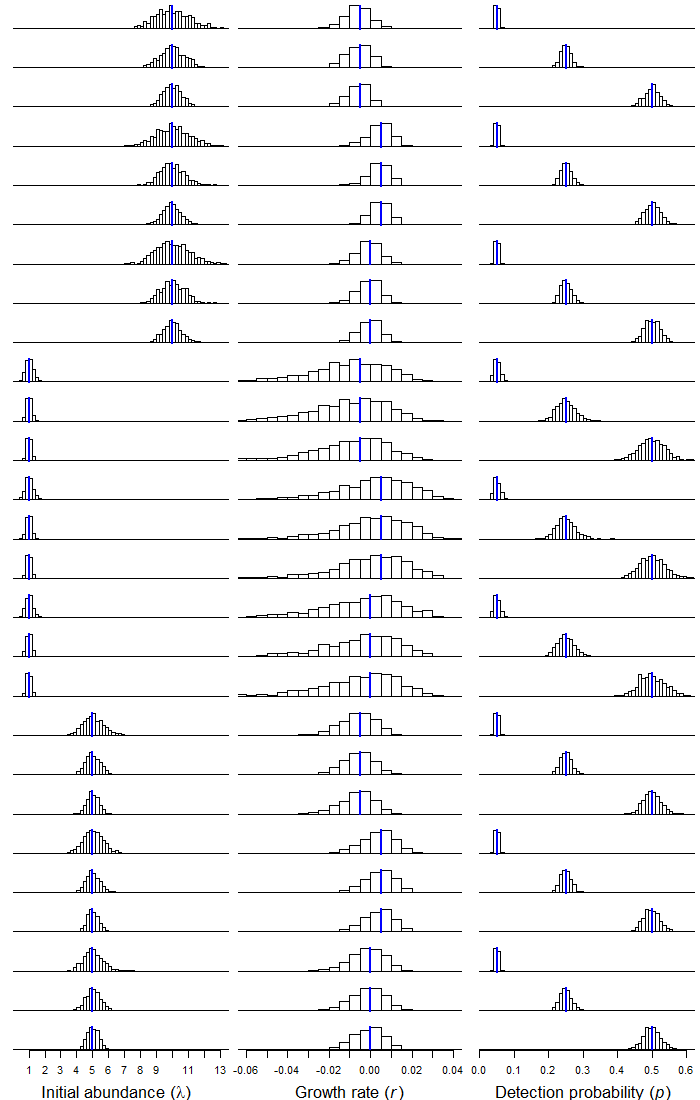
\includegraphics[height=8in]{figs/exp_hists}
\label{fig:exp_hists}
\end{figure}

\begin{figure}
\caption{}
  \centering
  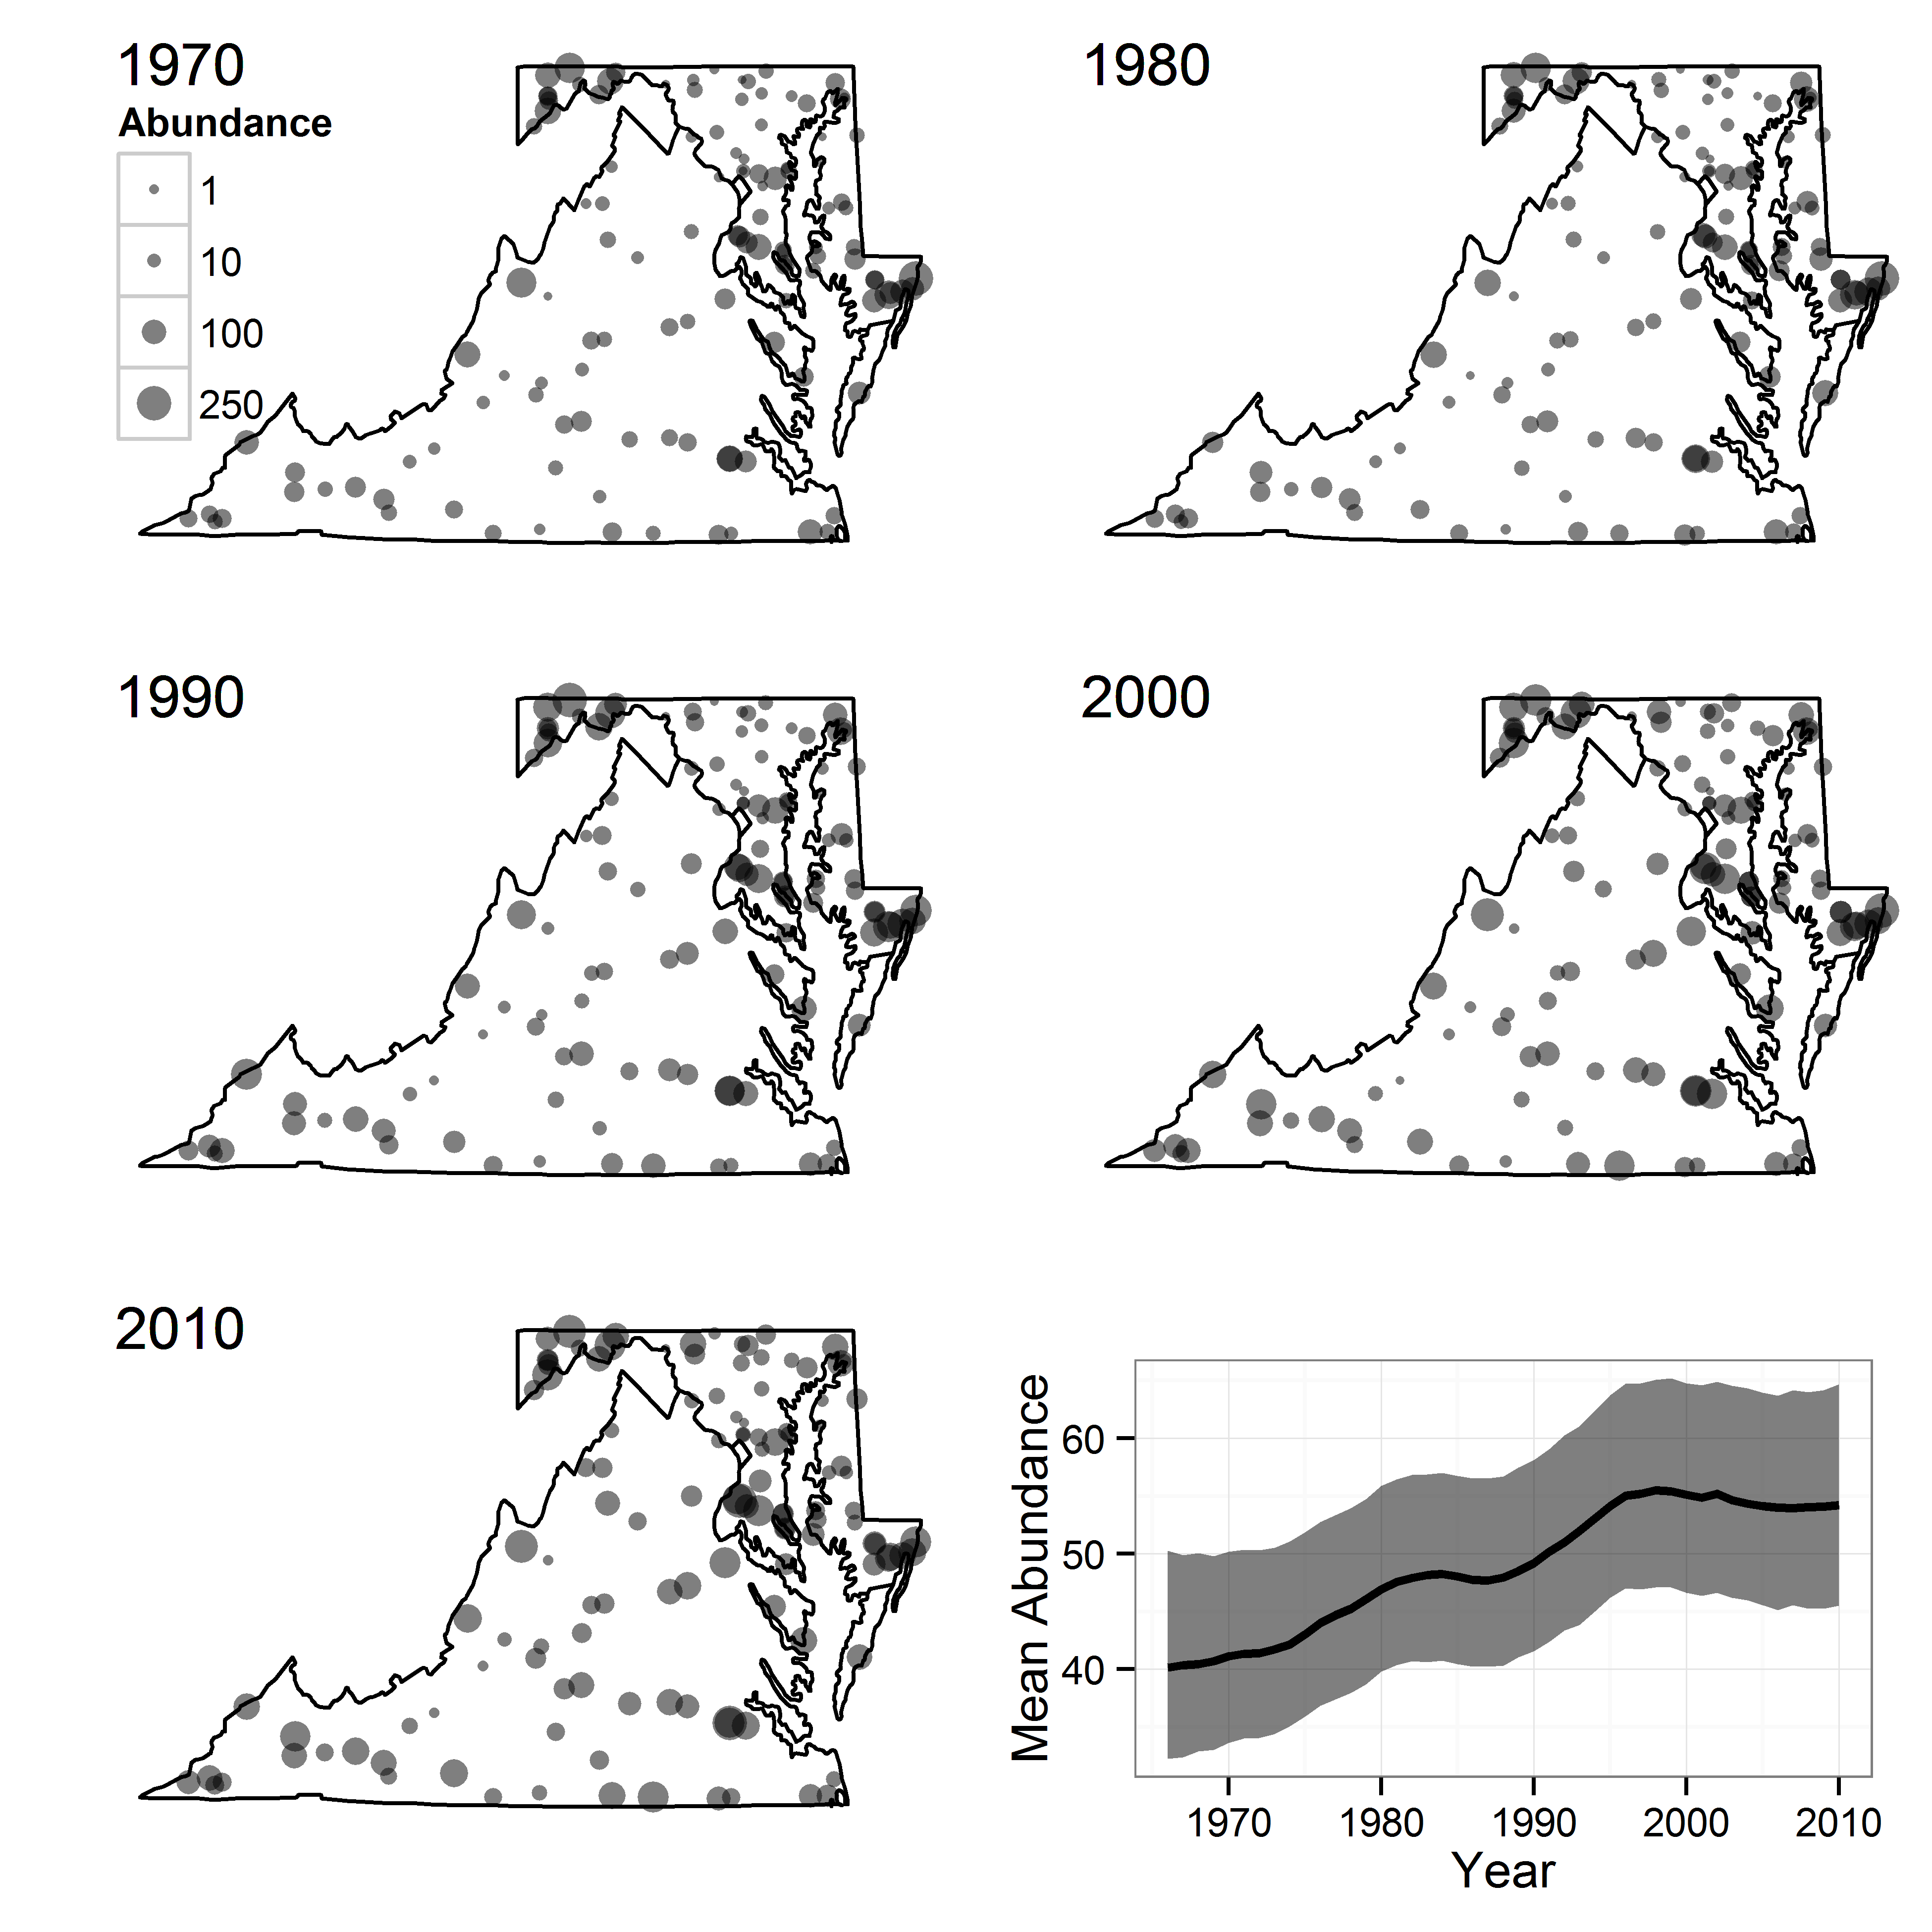
\includegraphics[width=6.6in]{figs/OVEN_N_by_route_year6}
\label{fig:oven_N}
\end{figure}
\end{flushleft}
\end{spacing}
\end{document}
